\documentclass[12pt]{article}
\usepackage[]{algorithm2e}
\usepackage{amsmath}
\usepackage{amsfonts,amssymb,amsthm,epsfig,epstopdf,titling,url,array}
\usepackage{geometry}
\usepackage{tikz}
\usetikzlibrary{arrows}
\usetikzlibrary{shapes,snakes}
\usepackage{array}
\usepackage{float}
\usepackage[utf8]{inputenc}
\usepackage[normalem]{ulem}
\useunder{\uline}{\ul}{}

\usepackage[figuresright]{rotating}
\usepackage{tikz}
\usepackage[margin=2cm]{caption}
\usepackage{xhfill}
\usepackage{listings}
\usepackage{float}
\usepackage{amsmath}
\usepackage{xcolor}
\usepackage{makecell}
\usetikzlibrary{arrows,positioning} 

\tikzset{
	%Define standard arrow tip
	>=stealth',
	%Define style for boxes
	box/.style={
		rectangle,
		rounded corners,
		draw=black, very thick,
		text width=20em,
		minimum height=5.5em,
		text centered},
	% Define arrow style
	edgeStyle/.style={
		->,
		thick}
}

\newcommand{\HRule}[1][\medskipamount]{\par
	\vspace*{\dimexpr-\parskip-\baselineskip+#1}
	\rule{15.5em}{0.4pt}\par
	\vspace*{\dimexpr-\parskip-.5\baselineskip+#1}}


\renewcommand{\baselinestretch}{1.25}

\geometry{
	a4paper,
	total={160mm,257mm},
	left=30mm,
	right=20mm,
	top=20mm,
	bottom=20mm,
}

\theoremstyle{definition}
\newtheorem{defn}{Definitie}[section]
\newtheorem{proposition}{Propozitie}[section]
\newtheorem{exmp}{Exemplu}[section]

%opening
\title{}
\author{}

\begin{document}
\begin{titlepage}
	\begin{center}
		\vspace{1cm}
		``ALEXANDRU IOAN CUZA" UNIVERSITY OF IAȘI
		\
		\\
		\begin{large}
			\textbf{FACULTY OF COMPUTER SCIENCE}\\
		\end{large}	
		\vspace{2.5cm}
		
\includegraphics{fii.png}
		\
		\\
		\vspace{1cm}
		Master's Thesis
		\begin{large}
			\
			\\
			\vspace{1.5cm}
			\textbf{Composition Algorithm for Relational Semantic Model}
		\end{large}
		\\
		\vspace{1.5cm}
		\textbf{by}
		\\
		\vspace{1.5cm}
		\textit{\textbf{Ștefania-Liana Țucăr}}
		\\
		\vspace{3cm}
		\textit{Master Programme: Advanced Studies in Computer Science}
		\\
		\textit{July, 2019}
		\\
		\vspace{3cm}
		\textbf{Scientific Coordinator}
		\textit{\textbf{Prof. Dr. Croitoru Cornelius}}
		
		
	\end{center}
\end{titlepage}
\newpage

\tableofcontents
\newpage


\section{Introduction}
Service Oriented Architectures are very popular these years as it is a modular architecture. Services usually have their specific functionality and more complex scenarios use the services as building blocks. This way the same implementation of a functionality can be used multiple times in different scenarios, this being an improvement in production time as well as resources utilization.
\\
%paragraful de sus cam vrajeala..de corectat! \\
Having a repository of web services, they can be combined in different ways to serve requests that otherwise could not be solved using only one service. As repository usually have a big number of services and requests should usually be answered fast, automating this process is a real need. This can be solved by automatic web service composition. \\ 
Among information about a specific service the following is of interest in the context of service composition: input parameters that can be used to call the service and preconditions (i.e. properties that objects used to instantiate the parameters should have); output parameters that are obtained after the service is called and postonditions (i.e. properties that are guaranteed that the output objects have). \\
Different models for representing services and matching parameters have been proposed in the context of web service composition. In the model presented WSC2005 competition the parameters are matched only by their names. The model is improved from the semantic point of view in the WSC2008 competition \cite{WSC2008} where parameters are described using concepts from an ontology. \\
%Cv sa zic si ca web-ul devine mai semantinc... \\

\subsection{Contribution}
A model that aims to leverage semantic information is proposed in \cite{paulRelational}. Parameters are described by concepts from an ontology and also by relations between them. Preconditions that enable calling a service as well as postconditions (properties satisfied by the output of the service call) are expressed by binary relations between parameters. This provides a significant improvement in the expressivity of the model. Thus the composition obtained after modeling real services and user queries in the proposed way is supposed to be more valuable than the ones provided after modeling in a more simplistic way, because more semantic information is used in this model. \\
In \cite{paulRelational} an algorithm for solving the composition problem (in the relational model) is described. A new version of the algorithm is presented in section \ref{algorithm} that proves to be faster and to obtain a shorter composition. In the new proposed algorithm the decision to call services is made tacking into consideration the semantic context of the objects thus resulting in a shorter composition and a faster algorithm. \\
%Cv optimizari..??? (astea poate trebuie mutate in concluzie?) \\
A more detailed description of the problem in the proposed model is presented in section \ref{problem}. A proposed algorithm for solving the web service composition problem under the proposed model is explained in section \ref{algorithm}.\\
In section \ref{evaluare} the testset generator that was implemented to evaluate the algorithm is described as well as results of the proposed algorithm on the generated testcases and on public testcases that were modified to be compatible with the proposed model.
 %aici de zis mai bn si mai frumos despre comparatii...\\
%	Relational wsc bla bla


\newpage
\section{Motivating Example}
Following is presented an example (presented also in \cite{paulRelational}) that showcases the increase in expressiveness of the proposed model compared to the models based only on a hierarchy of concepts. The enhancement comes from adding relations between objects/parameters and inference rules that can be used to deduct more relations between objects. \\
The scenario is described below. A teacher is trying to schedule a meeting at some collaborating university. The following information is provided: identifier of the person, university where the teacher works, and the name of the university he wants to visit. The person is an instance of \textbf{Person} concept and both universities are instances \textbf{University} concept. \\
Two inference rules are defined: \textbf{locatedAtWorkRule}: if \textbf{pers} is an employee of \textbf{univ} and \textbf{univ} is located at \textbf{location} then \textbf{pers} is located in \textbf{location}; \textbf{destinationGenRule} as described in the Figure \ref{fig:largeExample}.


\begin{figure*}[h!]
	\centering
	\vspace{1em}
	{
		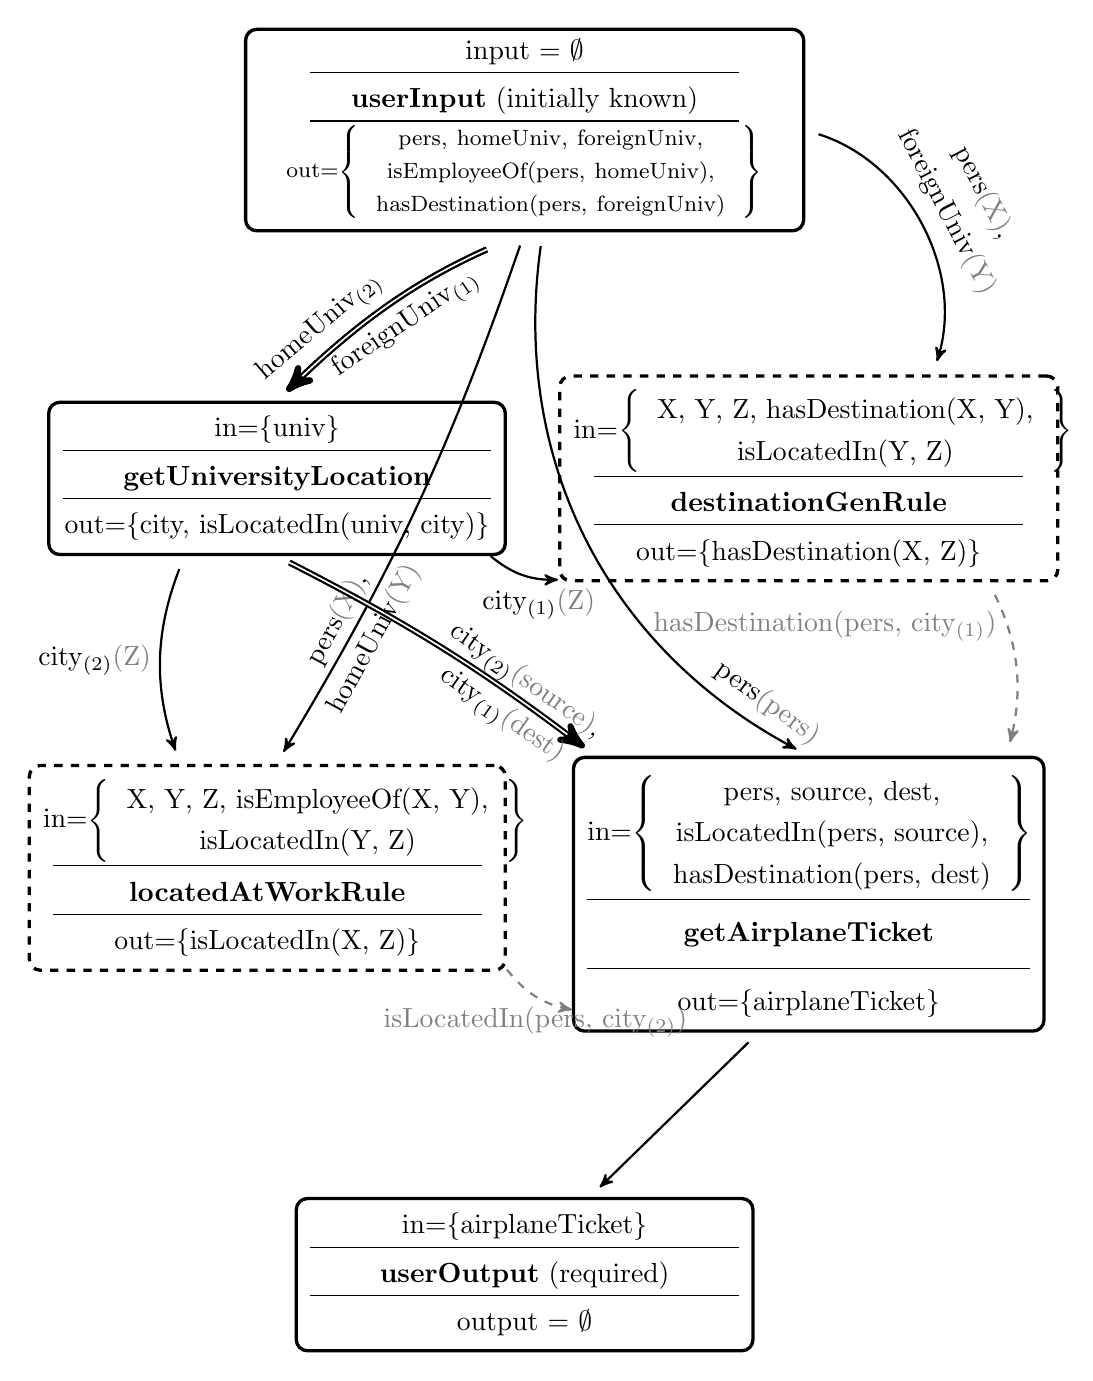
\begin{tikzpicture}	[x=0.45pt,y=0.45pt,yscale=1,xscale=1]
		
		%nodes
		\node[box, text width=19.5em] (input) {
			input = $\emptyset$\\
			\HRule[5pt]
			\textbf{userInput} (initially known)\\
			\HRule[5pt]
			\vspace{2pt}
			\footnotesize{out=$\left \{\begin{tabular}{c}pers, homeUniv, foreignUniv, \\ isEmployeeOf(pers, homeUniv), \\ hasDestination(pers, foreignUniv)\end{tabular}\right \}$}\\
		};
		
		\node[below=3cm of input] (dummy) {};
		
		\node[box, dashed, text width=16.2em, inner sep=5pt,below left =3.5cm and 0.1 cm of dummy] (locAtWorkNode) {
			in=$\left \{\begin{tabular}{c}X, Y, Z, isEmployeeOf(X, Y), \\ isLocatedIn(Y, Z)\end{tabular}\right \}$ \\
			\vspace{9pt}
			\HRule[5pt]
			\textbf{locatedAtWorkRule}\\
			\HRule[5pt]
			out=\{isLocatedIn(X, Z)\}\\
		};
		\draw (input.south) edge[edgeStyle, bend left=6, shorten <= 5pt, shorten >= 5pt] node[near end, sloped]{\begin{tabular}{c}pers\textcolor{gray}{(X)}, \\homeUniv\textcolor{gray}{(Y)}\end{tabular}} (locAtWorkNode.85);
		
		\node[box, text width=15.5em, inner sep=5pt,left =0.1 cm of dummy] (getUnivNode) {
			in=\{univ\}\\
			\HRule[5pt]
			\textbf{getUniversityLocation}\\
			\HRule[5pt]
			out=\{city, isLocatedIn(univ, city)\}\\
		};
		
		\node[box,  dashed, text width=17em, inner sep=5pt,right=0.3cm of dummy] (destGenNode) {
			in=$\left \{\begin{tabular}{c}X, Y, Z, hasDestination(X, Y), \\ isLocatedIn(Y, Z)\end{tabular}\right \}$\\
			\vspace{9pt}
			\HRule[5pt]
			\textbf{destinationGenRule}\\
			\HRule[5pt]
			out=\{hasDestination(X, Z)\}\\
		};
		\node[box, text width=16em, inner sep=5pt,below=2.2cm of destGenNode] (getAirplaneNode) {
			in=$\left \{ \begin{tabular}{c}pers, source, dest, \\ isLocatedIn(pers, source), \\ hasDestination(pers, dest)\end{tabular} \right \} $\\
			\hrulefill
			\\ \textbf{getAirplaneTicket} \\
			\vspace{-5pt}
			\hrulefill
			\\out=\{airplaneTicket\}\\
		};
		\node[box, text width=15.5em, inner sep=5pt,below =9cm of dummy] (output) {
			in=\{airplaneTicket\}\\
			\HRule[5pt]
			\textbf{userOutput} (required)\\
			\HRule[5pt]
			output = $\emptyset$\\
		};
		
		\draw (input.south) edge[edgeStyle, double, bend right=10,shorten <= 15pt, shorten >= 5pt] node[sloped, below] {foreignUniv$_{(1)}$} (getUnivNode.north) ;
		\draw (input.south) edge[edgeStyle, double, bend right=10,shorten <= 15pt, shorten >= 5pt] node[sloped, above, near end] {homeUniv$_{(2)}$} (getUnivNode.north) ;
		\draw (input.east) edge[edgeStyle, bend left=45,shorten <= 5pt, shorten >= 5pt] node[sloped, above] {\begin{tabular}{c} pers\textcolor{gray}{(X)},\\ foreignUniv\textcolor{gray}{(Y)}\end{tabular}} (destGenNode.40);
		\draw (getUnivNode.340) edge[edgeStyle, bend right=20] node[below, near end]{city$_{(1)}$\textcolor{gray}{(Z)}}  (destGenNode.202);
		\draw (getUnivNode.220) edge[edgeStyle,shorten <= 5pt, shorten >= 5pt, bend right = 20] node[left] {city$_{(2)}$\textcolor{gray}{(Z)}}  (locAtWorkNode.130);
		\draw (destGenNode.330) edge[edgeStyle, dashed, gray, bend left = 20,shorten <= 5pt, shorten >= 5pt] node[left, near start] {hasDestination(pers, city$_{(1)}$)} (getAirplaneNode.35);
		\draw (locAtWorkNode.337) edge[dashed, gray, edgeStyle, bend right=20] node[below]{isLocatedIn(pers, city$_{(2)}$)} (getAirplaneNode.206);
		\draw (input.280) edge[edgeStyle, bend right=35,shorten <= 5pt, shorten >= 5pt] node[very near end, above, sloped] {\hspace{10pt} pers\textcolor{gray}{(pers)}} (getAirplaneNode.north);
		\draw (getUnivNode.south) edge[edgeStyle,double, shorten <= 5pt, shorten >= 5pt, bend left=5] node[near end, sloped]{{\begin{tabular}{c}city$_{(2)}$\textcolor{gray}{(source)},\\city$_{(1)}$\textcolor{gray}{(dest)}\end{tabular}}} (getAirplaneNode.147);
		\draw (getAirplaneNode.250) edge[edgeStyle,shorten <= 5pt, shorten >= 5pt] (output.50);
		
		\end{tikzpicture}
	}
	\caption{Example motivating the need for relations and rules in composition language.\\ Service parameter types are not shown for simplicity.}
	\label{fig:largeExample}
\end{figure*} 

In Figure \ref{fig:largeExample}, solid boxes represent services and the user request (one for input - the initially known concepts and their relations, and one for the required output). Dashed boxes represent inference rules. Edges show information flow: solid edges - parameters and the dashed edges - relationships among them. Not all possible relations are used. Parameters are matched to rule variables (rule "parameters"), or other service parameters, based on the specification in gray in parenthesis. Multiple calls to the same service can be handled and are shown with double edges.

One composition representing a valid solution for the described instance would be the following list ordered list of service invocations:

\noindent \textbf{getInput}\big($\emptyset$\big) $\Longrightarrow$ pers, homeUniv, foreignUniv, isEmployeeOf(pers, homeUniv), hasDestination(pers, foreignUniv);

\noindent \textbf{getUniversityLocation}\big(homeUniv\big) $\Longrightarrow$ homeCity, isLocatedIn(homeUniv, homeCity); 

\noindent \textbf{getUniversityLocation}\big(foreignUniv\big) $\Longrightarrow$ foreignCity, isLocatedIn(foreignUniv, foreignCity);

The two cities: \emph{homeCity} and \emph{foreignCity} are differentiated based on their relations, the names are not relevant for the composition (there is no restriction on what names they get if they would be automatically created; i.e. any distinct strings would work).

\noindent \textbf{locatedAtWorkRule}\big(pers, homeUniv, homeCity, isEmployeeOf(pers, homeUniv), isLocatedIn(homeUniv, homeCity)\big) $\Longrightarrow$ isLocatedIn(pers, homeCity);

\noindent \textbf{destinationGenRule}\big(pers, foreignUniv, foreignCity, hasDestination(pers, foreignUniv), isLocatedIn( foreignUniv, foreignCity)\big) $\Longrightarrow$ hasDestination(pers, foreignCity); 

\noindent \textbf{getAirplaneTicket}\big(pers, homeCity, foreignCity, isLocatedIn(pers, homeCity), hasDestination(pers, foreignCity) $\Longrightarrow$ airplaneTicket;

In this example the possible need of different objects of the same type can be easily noticed - there are two different universities as instance of the same concepts, but each has a different semantic context described by relations: person \textbf{isEmployeeOf} Univ1 and person \textbf{hasDestination} Univ2.

The example could be modified to show the use of a hierarchy of objects, but for the sake of simplicity it is kept this way. It could for example have a hierarchy of concepts where University is a subconcept of Builing and the service getUniversityLocation is modified as getBuildingLocation; so the getBuildingLocation could be called with university as input parameter for building because university is a building (according to the hierarchy of concepts).

\newpage
\section{Problem Description} \label{problem}
	Given a repository of services and an user query the objective is to find a composition that can answer the query.  Each service is described by an identifier, a lists of input parameters, a list of preconditions (relations that need to be satisfied to call the service), a list of output parameters and a list of postconditions. \\
	For representing the possible types and relations between objects (and parameters) an ontology is defined. The ontology is defined as a hierarchy of concepts, each concept being identified by its' name; a list of relation names and a list of inference rules. \\
	A composition is an ordered list of service invocations. More precisely it is a list of service identifiers and if more details are useful, the objects used to call each service can be included.
	\subsection {Problem Definition}
	Let $Names$ be a list of all possible identifiers used to differentiate between concepts, parameters, services. It can be simply a list of strings over a predefined alphabet.
	\paragraph{Concepts and Parameters} 
		Let $ \mathcal{C} $ be the set of all concepts that can be used to describe object and parameter types. Each concept is identified by a name. \\
		$Params \subseteq Names \times \mathcal{C}$. Let $Params$ be the set of all possible parameters. A parameter has a name and a type from the concepts hierarchy. 
	\par
	\paragraph{Ontology} $Ontology = (Hierarchy, Relations, Rules);$ \\
		$ Hierarchy = (\mathcal{C}, subType) $ is a tree of concepts. \\
		$ subType \subseteq \mathcal{C} \times \mathcal{C}$ transitive acyclic relation that describes the types hierarchy. \\  
		$ Relations \subseteq \mathcal{P}(Names)$, where $\mathcal{P}$ represents the power set.  \\
		$ Rules = $ set of inference rules over Relations.% aici trebuie rescris!!! $ Relations \subseteq Names \times \mathcal{C} \times \mathcal{C}$ is a set of binary relations
	\par
	\paragraph{Repository} $Rep = \{ \mathcal{S}erv_1, ..., \mathcal{S}erv_n \}$. \\
		The \textit{repository} is a set of services identified by names.\\
		$\mathcal{S}erv = (name, inputParams, outputParams, preConditions, postConditions); \\
		inputParams, outputParams \subseteq \mathcal{P}arams;\\ 
		preConditions \subseteq \mathcal{P}(Relation \times inputParams \times inputParams)$ \\
		$postConditions \subseteq \mathcal{P}(Relation \times Par);$, where 
		$Par = (inputParams \cup outputParams) \times (inputParams \cup outputParams) \setminus
		(inputParams \times inputParams );$\\\\
		Each \textit{service} is defined by a name, two lists of parameters (input and output) and two lists of relations between parameters (preconditions and postconditions). The preconditions are relations only between input parameters while the postconditions are relations between input and output parameters or output and output parameters.
	\par
	
	\paragraph{Query}
		$ Query = ( providedParams, requiredParams, providedRels, requiredRels ); \\ 
		  providedParams, requiredParams \subseteq Params;$ \\ 
		  $providedRels \subseteq \mathcal{P}(Relation \times providedParams \times providedParams)$ \\
		  $requiredRels \subseteq \mathcal{P}(Relation \times Par);$, where 
		  $Par = (providedParams \cup requiredParams) \times (providedParams \cup requiredParams) \setminus (providedParams \times providedParams );$\\
		  The query is defined by the provided parameters and relations which describe the types of the objects provided and the relations between them and by the required parameters and relations which describes the types and relations that the objects obtained after the composition need to satisfy. \\ %de reformulat
		  It has a similar structure with a service, but replacing input parameters/relations with provided parameters/relations and output parameters/ relations with required parameters/ relations. Their meaning is somehow reversed. 
	\par
	
	\paragraph{Knowledge}
		$ Knowledge = (Objects, Relations); \\
		  Objects = \{Obj_1, ..., Obj_k\} \subseteq Names \times Concepts; \\
		  Relations \subseteq Relations \times Objects \times Objects$. \\
		The Knowledge is a tuple formed by a set of objects and a set of relations defined on those objects. It represents the set of all objects obtained after service calls or directly provided from the user query together with the known relations that hold between objects.\\
		Each object has a specific type (defined by a concept) and a name. There can be multiple objects of the same type.
	\par
	
	\paragraph{Service Call}
		$ ServCall = (Serv, objAssignation); \\
		  Serv = (name, inputParams, outputParams, preConds, postConds); \\
		  objAssignation : inputParams \to Knowledge.$ \\
		A service can be called assigning an object to each of its input parameters. The objects assigned need to "match". An object matches to a parameter if the type of the object is equal or more particular to the type of the parameter (according to the types hierarchy defined in ontology). Besides this condition the objects need to satisfy all the preconditions the service defines so all the relations from preconditions between parameters need to hold for the objects assigned to parameters.\\
		%?ce se intampla dupa ce fac un call???
		The service together with the objects assigned for the input parameters form a "service call".
	\par
	
	\paragraph{Composition}
		$ Comp = (ServCall_1, ..., ServCall_m)$; \\
		A composition is an ordered list of service calls (services and objects used to call the services). Each service call needs to be possible i.e. objects from knowledge can be assigned to all input parameters.
	\par
	
	%Pe aici tre sa descriu mai mult si mai formal ce inseamna compozitie... sa pot face call la un serviciu (in compozitie) si cu chestiile pe care le obtin dupa.. si ce inseamna ca compozitia rezolva query-ul
	
	\paragraph{Problem Instance}
	Input: $(Rep, Ontology, Query)$;\\
	Output: $Composition$ that solves the $Query$. \\ %sa explic ce inseamna ca rezolva query-ul
	Given a repository of web services, the ontology and an user query, a valid composition that solves the user query should be returned. The composition solves the query if all the required parameters can be found in the knowledge obtained after all service calls (within the composition) are made. Meaning that for every required parameter (from query) a corresponding object with matching type needs to be found in the knowledge. Besides this condition, the required relations (from query) between parameters need to hold for objects used to instantiate them.
	\par
	
\newpage
\section{Algorithm} \label{algorithm}
	\subsection{Algorithm Description}
	\subsubsection{Main Idea}
	During the construction of the composition a set of objects and relations between objects is kept in memory. This set is called "knowledge".\\
	In the beginning of the algorithm the knowledge is formed only of the objects and relations from the query provided information (query.providedParams and query.providedRels) - this being the information provided by the user in order to obtained the desired information (query.required). \\
	As the composition grows (i.e. services can be called and added to composition and new objects and relations are obtained as a consequence) objects and relations are added to the knowledge until no more services can be called or until the query can be answered (i.e. the required parameters and relations are obtained).\\
	To handle inference rules in a simple manner, in the initialization phase fake services are added in the repository. For each inference rule a corresponding fake service is created and added in the repository. This step does not significantly increase the execution time of the algorithm as the number of inference rules is usually smaller than the number of initial services.\\
	During all the following algorithm the repository, ontology, query, knowledge and composition are considered global values (for writing simplicity).\\
	
	\begin{algorithm}[H]
		\KwData{repository, ontology, query}
		\KwResult{Composition that solves the query if it finds one; "Not Solved" otherwise.}
		initialize data structures and create fake services for inference rules\;
			
		$changed \gets True$\;
		
		\While{$\neg canAnswerQuery(query)$ And $changed = True$}{
			($changed$ , $composition$, $knowledge$) $\gets constructionPhase()$\;
		}
		\If{$canAnswerQuery(query)$}{
			\Return $composition$\; % aici sa vad ce returnez
		}\Else{
			\Return $Not\ Solved$\;
		}
		\caption{Main function}
	\end{algorithm}

	During the algorithm there is a need to know if the query is solved. Multiple calls to this function are made. \\
	The query is said to be solved if objects with the required properties (i.e. proper types and relations between them) can be found in the knowledge. A fake service is constructed with the property that being able to call that service is equivalent to solving the query. The service is not added in the repository. It is just used for checking if the query is solved.\\
	The service has as input parameters all parameters from the query and as preconditions all the relations from the query. Despite the fact that query.providedParams are always in the knowledge they still need to be added in the fake service input parameters. This happens because some of the required relations from the query can be relations between input and output parameters. So to be able to check all required relations, all the parameters from the query need to be added as service input parameters.\\
	If the constructed fake service is callable, then the query can be answered (and the algorithm will stop). \\
	
	\begin{algorithm}[H]
		\KwData{query, knowledge}
		\KwResult{$True$ if the query is solved; $False$ otherwise.}
		
		\SetKwFunction{FMain}{canAnswerQuery}
		\SetKwProg{Fn}{Function}{:}{}
		\Fn{\FMain{$query, knowledge$}}{
			$serv \gets newService()$ \;
			$serv.inParams \gets query.providedParams \ \cup \ query.requiredParams$ \;
			$serv.preconditions \gets query.providedRels \ \cup \ query.requiredRels$ \;
			$serv.outParams \gets \emptyset$ \;
			$serv.postconditions \gets \emptyset$ \;
			\Return $canCallService(serv, knowledge)$ \;
		}
		\caption{Function that checks if the query is solved using objects in the knowledge}
	\end{algorithm}
	\subsubsection{Construction Phase}
	In the construction phase all the services (including the fake ones created for handling the inference rules) from the repository are iterated and for each service all the possible calls are searched. A service can be called multiple times with different input parameters. From all the possible calls of a service only the ones that provide "useful" information are added to the composition.\\
	If at least one service call was added in the composition, the composition is updated accordingly and the function returns "True" (for the calling function to continue the algorithm run).
	
	\begin{algorithm}[H]
		\KwData{repository, ontology, query}
		\KwResult{True if services were added to the composition; False otherwise}
		\SetKwFunction{FMain}{constructionPhase}
		\SetKwProg{Fn}{Function}{:}{}
		\Fn{\FMain{}}{
		
		$compositionUpdated \gets False$ \;
		\ForEach{$service \in repository$}{
			$possibleCalls \gets searchForPossibleCalls(service)$ \;
			\ForEach{$servCall \in possibleCalls$}{
				\If{$providesUsefulInformation(servCall)$}{
					$makeCall(servCall)$ \;
					$compositionUpdated \gets True$ \;	
				}
			}	
		}
		\Return $compositionUpdated$ %de vazut ce e la return si ce e global. composition poate il fac global
		}
		\caption{constructionPhase}
	\end{algorithm}
	% sa zic ca asta e o optimizare si s-o laud..probabil datorita la faza asta algoritmu meu obtine putine servicii in compozitie
	When a service call is made new objects and relations corresponding with the service output and postconditions are created and added in the knowledge. \\
	If for all the new objects that would be created after a service call other objects that are similar or better than them already exist in the knowledge than the service call should not be made. If the service call would be made than no useful result is obtained, but the knowledge size would grow. \\
	A service call is useless if all the new objects obtained are "semantically similar" with other already present in the knowledge. To obtain the semantic context of an object the connected component from the knowledge that would contain the object (if added in the knowledge) needs to be extracted. \\
	%cam ameteala probabil pe aici... sa explic mai clar
	To check if the service call provides useful information a fake service is created and checked if it can be called. The fake service has as input parameters and preconitions the semantic context of all objects obtained after the service call (i.e. the connected components of the objects as explained above). \\
	If the fake service created (but not added to the repository) can be called, then the service call would be useless (all the information obtained already exists in the knowledge).
	
	\begin{algorithm}[H]
		\KwData{servCall, knowledge}
		\KwResult{$True$ if the service call provides useful information; $False$ otherwise.}
		\SetKwFunction{FMain}{providesUsefulInformation}
		\SetKwProg{Fn}{Function}{:}{}
		\Fn{\FMain{$servCall$}}{
			$params \gets servCall.service.inParams \cup servCall.service.outParams$ \;
			$objects \gets \{obj\ \vert\ obj = servCall.assignment[param]; param \in params \}$ \;
			$rels \gets \{ rel\ \vert\ rel \in knowledge; rel.o1, rel.o2 \in objects \}$ \;
			$serv \gets newService()$ \;
			$serv.inParams \gets \{ new Param(type = obj.type)\ \vert\ obj \in objects  \}$ \;
			$serv.preconditions \gets \{ new Relation(rel.name, o1=x, o2=y) \ \vert $\\$ \ rel\in rels; x = paramToObj[rel.x]; y= paramToObj[rel.y] \}$ \; %???????aici probabil e cam dubios..de verificat!
			$serv.outParams \gets \emptyset$ \;
			$serv.postconditions \gets \emptyset$ \;
			\Return $\neg canCallService(serv, knowledge)$ \;
		}
		\caption{Function that checks if the service call provides "new" information}
	\end{algorithm}

	\subsubsection{Search for service calls}
	Given a service, the task of finding all possible service calls means finding all combinations of objects that can be used as input parameters for the service. This involves finding for each input parameter a corresponding object that has a type that is equal or more general with the parameter type. Besides this condition regarding the types, the objects found need to satisfy all declared preconditions from the service definition (i.e. all relations from preconditions need to hold between corresponding objects used to call the service). \\
	This problem is equivalent to finding all labeled subgraph isomorphisms in the following constructed problem instance: 
	\begin{itemize}
		\item the "pattern" graph: for each input parameter a corresponding vertex with the label equal to the type of the parameter. For each relation from preconditions a corresponding directed edge between vertices correspondent to parameters involved in relation is added in the graph.
		\item the graph in which the pattern searched: for each object in the knowledge a vertex with the label equal to the type of the parameter. For each relation that holds between objects from the knowledge a corresponding directed edge is added in the graph.
	\end{itemize}

	% chestii despre problema cu citari...
	The problem is known to be NP-Complete (as stated for example in \cite{NPComplete}). 
	
	A backtracking procedure was implemented to solve this problem. For each input parameter all the known objects of matching types are iterated and all the preconditions involving the parameter and another parameter that has an object already chosen are checked. If all these relations match, than the object is chosen for this parameter and the backtracking procedure is recursively called for the next parameters.
	%mai multe detalii..hashuri acolo unde trebuie...
	%aici sa mai zic ca optimizarile is relevante fiindca functia asta e apelata de multe ori si dureaza cam cel mai mult din algoritm. optimizari: mapuri...sortare param dupa grad? faza cu prunning de la ullman sau ??? .... 
	%sa pun pseudocod la fct de generare!!!
	% tre sa mai scriu si makeCall(serviceCall). Sa mai vad si ce alte fct mai trebuie scrise
	% fct care creaza servicii pt inference rules? poate o descriu doar pe scurt in cuvinte (faza cu root).
	% search for possible calls and can call service!! asta e baza. de descris si cu subgraph isomorphism etc....
	\newpage
	\section{Evaluation of the algorithm} \label{evaluare}
		%de zis ca se masoara timpii dupa bostrapping process (si citare..)
		
		\subsection{Testset Generator}
		In order to evaluate the algorithm presented in Chapter \ref{algorithm}, a test set generator was implemented. The generator is a nondeterministic program that produces: a repository, ontology and user query that has a high probability of being solvable. These elements form a problem instance. \\
		In the first phase of generation, it produces the repository: a set of services that have the property that a composition that uses more than one service can be produced using them.\\
		To generate such services, the following observation is useful: as the composition grows (i.e services are "called" meaning that they are added in the composition), new objects and relations between objects are obtained so the knowledge is enhanced. So, to generate the repository, we start by generating and saving stages of the knowledge (that would correspond to the knowledge growth as services ar added to the composition). \\
		To obtain the repository we need to create services that can generate these stages. Between each two consecutive stages $K_i$, $K_{i+1}$ we generate a "layer" of services with each service having as input parameters objects and relations between them from $K_i$ and output parameters in a similar way from $K_{i+1}$, as shown in Figure \ref{fig:testgenerator}. The repository is formed by all the services produced in this step (saved in an arbitrary order). \\
		The ontology is formed by all the concepts produced while generating the knowledge stages. To obtain a taxonomy of concepts, they are arranged in a random hierarchy having a most general concept as the root of the produced tree. Relations and inference rules are generated and added to the ontology. \\ 
		The user query is generated also using the knowledge stages: the provided parameters and relations of the query are a subset of the first stage of the knowledge, while the required parameters and relations are a subset of the last stage. \\
		To make the problem instance harder to solve more concepts, services and relations are added in the repository and ontology. This can be viewed as a noise adding phase.\\
		%sa leg figura asta de ce e scris mai sus si poate sa modific putin cu stage1, ..., stagen si poate sa mai fac una si cu query...mhm..
		
		\begin{figure}[H]
			\centering
			\tikzset{every picture/.style={line width=0.75pt}} %set default line width to 0.75pt        
			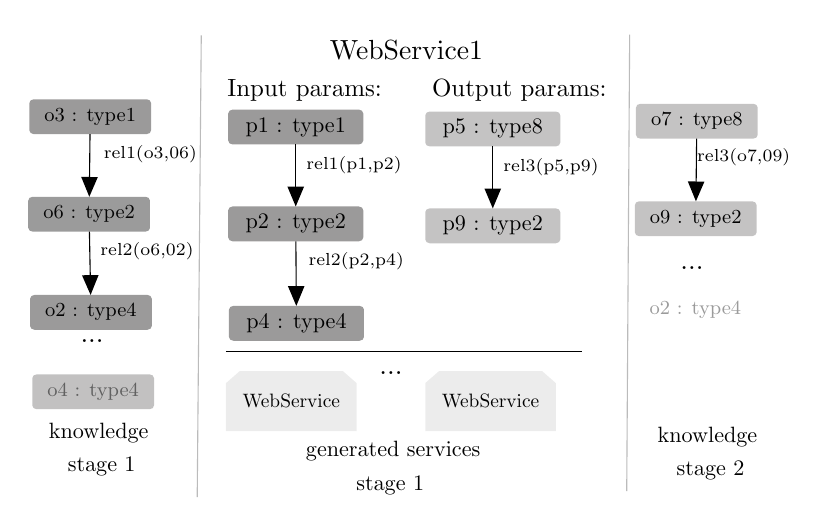
\begin{tikzpicture}[x=0.80pt,y=0.70pt,yscale=-1,xscale=1]
			%uncomment if require: \path (0,356); %set diagram left start at 0, and has height of 356
			
			%Snip Same Side Corner Rect [id:dp18629105681749092] 
			\draw  [draw opacity=0][fill={rgb, 255:red, 236; green, 236; blue, 236 }  ,fill opacity=1 ] (96.5,204.2) -- (102.7,198) -- (149.3,198) -- (155.5,204.2) -- (155.5,229) -- (155.5,229) -- (96.5,229) -- (96.5,229) -- cycle ;
			%Snip Same Side Corner Rect [id:dp8953411168142174] 
			\draw  [draw opacity=0][fill={rgb, 255:red, 236; green, 236; blue, 236 }  ,fill opacity=1 ] (186.5,204.2) -- (192.7,198) -- (239.3,198) -- (245.5,204.2) -- (245.5,229) -- (245.5,229) -- (186.5,229) -- (186.5,229) -- cycle ;
			%Straight Lines [id:da6104885642158018] 
			\draw    (96.5,188) -- (257.5,188) ;
			
			
			%Straight Lines [id:da29245072761199853] 
			\draw [color={rgb, 255:red, 187; green, 187; blue, 187 }  ,draw opacity=1 ]   (278.83,24.33) -- (277.5,260) ;
			
			
			%Straight Lines [id:da7469857558563573] 
			\draw [color={rgb, 255:red, 187; green, 187; blue, 187 }  ,draw opacity=1 ]   (85.33,24.67) -- (83.5,263) ;
			
			% Text Node
			\draw  [draw opacity=0]  (127.5,23) .. controls (127.5,21.9) and (128.4,21) .. (129.5,21) -- (226.5,21) .. controls (227.6,21) and (228.5,21.9) .. (228.5,23) -- (228.5,41) .. controls (228.5,42.1) and (227.6,43) .. (226.5,43) -- (129.5,43) .. controls (128.4,43) and (127.5,42.1) .. (127.5,41) -- cycle  ;
			\draw (178,32) node [scale=1] [align=left] { WebService1};
			% Text Node
			\draw  [draw opacity=0][fill={rgb, 255:red, 155; green, 154; blue, 154 }  ,fill opacity=1 ]  (97.5,65) .. controls (97.5,63.9) and (98.4,63) .. (99.5,63) -- (156.5,63) .. controls (157.6,63) and (158.5,63.9) .. (158.5,65) -- (158.5,79) .. controls (158.5,80.1) and (157.6,81) .. (156.5,81) -- (99.5,81) .. controls (98.4,81) and (97.5,80.1) .. (97.5,79) -- cycle  ;
			\draw (128,72) node [scale=0.8] [align=left] {p1 : type1};
			% Text Node
			\draw  [draw opacity=0][fill={rgb, 255:red, 155; green, 154; blue, 154 }  ,fill opacity=1 ]  (97.5,115) .. controls (97.5,113.9) and (98.4,113) .. (99.5,113) -- (156.5,113) .. controls (157.6,113) and (158.5,113.9) .. (158.5,115) -- (158.5,129) .. controls (158.5,130.1) and (157.6,131) .. (156.5,131) -- (99.5,131) .. controls (98.4,131) and (97.5,130.1) .. (97.5,129) -- cycle  ;
			\draw (128,122) node [scale=0.8] [align=left] {p2 : type2};
			% Text Node
			\draw  [draw opacity=0][fill={rgb, 255:red, 155; green, 154; blue, 154 }  ,fill opacity=1 ]  (97.83,166.33) .. controls (97.83,165.23) and (98.73,164.33) .. (99.83,164.33) -- (156.83,164.33) .. controls (157.94,164.33) and (158.83,165.23) .. (158.83,166.33) -- (158.83,180.33) .. controls (158.83,181.44) and (157.94,182.33) .. (156.83,182.33) -- (99.83,182.33) .. controls (98.73,182.33) and (97.83,181.44) .. (97.83,180.33) -- cycle  ;
			\draw (128.33,173.33) node [scale=0.8] [align=left] {p4 : type4};
			% Text Node
			\draw  [draw opacity=0][fill={rgb, 255:red, 155; green, 154; blue, 154 }  ,fill opacity=1 ]  (7.67,59.67) .. controls (7.67,58.56) and (8.56,57.67) .. (9.67,57.67) -- (60.67,57.67) .. controls (61.77,57.67) and (62.67,58.56) .. (62.67,59.67) -- (62.67,73.67) .. controls (62.67,74.77) and (61.77,75.67) .. (60.67,75.67) -- (9.67,75.67) .. controls (8.56,75.67) and (7.67,74.77) .. (7.67,73.67) -- cycle  ;
			\draw (35.17,66.67) node [scale=0.8,color={rgb, 255:red, 2; green, 2; blue, 2 }  ,opacity=1 ] [align=left] {{\small o3 : type1}};
			% Text Node
			\draw  [draw opacity=0][fill={rgb, 255:red, 155; green, 155; blue, 155 }  ,fill opacity=1 ]  (7.17,110) .. controls (7.17,108.9) and (8.06,108) .. (9.17,108) -- (60.17,108) .. controls (61.27,108) and (62.17,108.9) .. (62.17,110) -- (62.17,124) .. controls (62.17,125.1) and (61.27,126) .. (60.17,126) -- (9.17,126) .. controls (8.06,126) and (7.17,125.1) .. (7.17,124) -- cycle  ;
			\draw (34.67,117) node [scale=0.8,color={rgb, 255:red, 5; green, 5; blue, 5 }  ,opacity=1 ] [align=left] {{\small o6 : type2}};
			% Text Node
			\draw  [draw opacity=0][fill={rgb, 255:red, 155; green, 154; blue, 154 }  ,fill opacity=1 ]  (8,160.67) .. controls (8,159.56) and (8.9,158.67) .. (10,158.67) -- (61,158.67) .. controls (62.1,158.67) and (63,159.56) .. (63,160.67) -- (63,174.67) .. controls (63,175.77) and (62.1,176.67) .. (61,176.67) -- (10,176.67) .. controls (8.9,176.67) and (8,175.77) .. (8,174.67) -- cycle  ;
			\draw (35.5,167.67) node [scale=0.8,color={rgb, 255:red, 2; green, 2; blue, 2 }  ,opacity=1 ] [align=left] {{\small o2 : type4}};
			% Text Node
			\draw (62.33,86.17) node [scale=0.9] [align=left] {{\scriptsize rel1(o3,06)}};
			% Text Node
			\draw (60.83,136.17) node [scale=0.9] [align=left] {{\scriptsize rel2(o6,02)}};
			% Text Node
			\draw (155.33,141.17) node [scale=0.9] [align=left] {{\scriptsize rel2(p2,p4)}};
			% Text Node
			\draw (154.33,91.5) node [scale=0.9] [align=left] {{\scriptsize rel1(p1,p2)}};
			% Text Node
			\draw  [draw opacity=0][fill={rgb, 255:red, 196; green, 195; blue, 195 }  ,fill opacity=1 ]  (281.67,62) .. controls (281.67,60.9) and (282.56,60) .. (283.67,60) -- (334.67,60) .. controls (335.77,60) and (336.67,60.9) .. (336.67,62) -- (336.67,76) .. controls (336.67,77.1) and (335.77,78) .. (334.67,78) -- (283.67,78) .. controls (282.56,78) and (281.67,77.1) .. (281.67,76) -- cycle  ;
			\draw (309.17,69) node [scale=0.8,color={rgb, 255:red, 0; green, 0; blue, 0 }  ,opacity=1 ] [align=left] {{\small o7 : type8}};
			% Text Node
			\draw  [draw opacity=0][fill={rgb, 255:red, 196; green, 195; blue, 195 }  ,fill opacity=1 ]  (281.17,112.33) .. controls (281.17,111.23) and (282.06,110.33) .. (283.17,110.33) -- (334.17,110.33) .. controls (335.27,110.33) and (336.17,111.23) .. (336.17,112.33) -- (336.17,126.33) .. controls (336.17,127.44) and (335.27,128.33) .. (334.17,128.33) -- (283.17,128.33) .. controls (282.06,128.33) and (281.17,127.44) .. (281.17,126.33) -- cycle  ;
			\draw (308.67,119.33) node [scale=0.8,color={rgb, 255:red, 0; green, 0; blue, 0 }  ,opacity=1 ] [align=left] {{\small o9 : type2}};
			% Text Node
			\draw (330.33,87.5) node [scale=0.9] [align=left] {{\scriptsize rel3(o7,09)}};
			% Text Node
			\draw  [draw opacity=0][fill={rgb, 255:red, 196; green, 195; blue, 195 }  ,fill opacity=1 ]  (186.5,66) .. controls (186.5,64.9) and (187.4,64) .. (188.5,64) -- (245.5,64) .. controls (246.6,64) and (247.5,64.9) .. (247.5,66) -- (247.5,80) .. controls (247.5,81.1) and (246.6,82) .. (245.5,82) -- (188.5,82) .. controls (187.4,82) and (186.5,81.1) .. (186.5,80) -- cycle  ;
			\draw (217,73) node [scale=0.8] [align=left] {p5 : type8};
			% Text Node
			\draw  [draw opacity=0][fill={rgb, 255:red, 196; green, 195; blue, 195 }  ,fill opacity=1 ]  (186.5,116) .. controls (186.5,114.9) and (187.4,114) .. (188.5,114) -- (245.5,114) .. controls (246.6,114) and (247.5,114.9) .. (247.5,116) -- (247.5,130) .. controls (247.5,131.1) and (246.6,132) .. (245.5,132) -- (188.5,132) .. controls (187.4,132) and (186.5,131.1) .. (186.5,130) -- cycle  ;
			\draw (217,123) node [scale=0.8] [align=left] {p9 : type2};
			% Text Node
			\draw (243.33,92.5) node [scale=0.9] [align=left] {{\scriptsize rel3(p5,p9)}};
			% Text Node
			\draw (132,53) node [scale=0.9] [align=left] {Input params:};
			% Text Node
			\draw (229,53) node [scale=0.9] [align=left] {Output params:};
			% Text Node
			\draw  [draw opacity=0]  (281,159.33) .. controls (281,158.23) and (281.9,157.33) .. (283,157.33) -- (334,157.33) .. controls (335.1,157.33) and (336,158.23) .. (336,159.33) -- (336,173.33) .. controls (336,174.44) and (335.1,175.33) .. (334,175.33) -- (283,175.33) .. controls (281.9,175.33) and (281,174.44) .. (281,173.33) -- cycle  ;
			\draw (308.5,166.33) node [scale=0.8,color={rgb, 255:red, 155; green, 155; blue, 155 }  ,opacity=1 ] [align=left] {{\small o2 : type4}};
			% Text Node
			\draw (126,213.5) node [scale=0.7] [align=left] {WebService};
			% Text Node
			\draw (216,213.5) node [scale=0.7] [align=left] {WebService};
			% Text Node
			\draw (36,182.67) node  [align=left] {...};
			% Text Node
			\draw (171,199) node  [align=left] {...};
			% Text Node
			\draw (307,145) node  [align=left] {...};
			% Text Node
			\draw (39,238.33) node [scale=0.8] [align=left] {knowledge\\\hspace{0.3cm}stage 1};
			% Text Node
			\draw (314,240.67) node [scale=0.8] [align=left] {knowledge\\\hspace{0.3cm}stage 2};
			% Text Node
			\draw (172,248) node [scale=0.8] [align=left] {generated services\\\hspace{0.8cm}stage 1};
			% Text Node
			\draw  [draw opacity=0][fill={rgb, 255:red, 194; green, 193; blue, 193 }  ,fill opacity=1 ]  (9,201.67) .. controls (9,200.56) and (9.9,199.67) .. (11,199.67) -- (62,199.67) .. controls (63.1,199.67) and (64,200.56) .. (64,201.67) -- (64,215.67) .. controls (64,216.77) and (63.1,217.67) .. (62,217.67) -- (11,217.67) .. controls (9.9,217.67) and (9,216.77) .. (9,215.67) -- cycle  ;
			\draw (36.5,208.67) node [scale=0.8,color={rgb, 255:red, 97; green, 97; blue, 97 }  ,opacity=1 ] [align=left] {{\small o4 : type4}};
			% Connection
			\draw    (35.08,75.67) -- (34.78,106) ;
			\draw [shift={(34.76,108)}, rotate = 270.57] [fill={rgb, 255:red, 0; green, 0; blue, 0 }  ][line width=0.75]  [draw opacity=0] (8.93,-4.29) -- (0,0) -- (8.93,4.29) -- cycle    ;
			
			% Connection
			\draw    (34.81,126) -- (35.32,156.67) ;
			\draw [shift={(35.35,158.67)}, rotate = 269.06] [fill={rgb, 255:red, 0; green, 0; blue, 0 }  ][line width=0.75]  [draw opacity=0] (8.93,-4.29) -- (0,0) -- (8.93,4.29) -- cycle    ;
			
			% Connection
			\draw    (128,81) -- (128,111) ;
			\draw [shift={(128,113)}, rotate = 270] [fill={rgb, 255:red, 0; green, 0; blue, 0 }  ][line width=0.75]  [draw opacity=0] (8.93,-4.29) -- (0,0) -- (8.93,4.29) -- cycle    ;
			
			% Connection
			\draw    (128.06,131) -- (128.26,162.33) ;
			\draw [shift={(128.27,164.33)}, rotate = 269.63] [fill={rgb, 255:red, 0; green, 0; blue, 0 }  ][line width=0.75]  [draw opacity=0] (8.93,-4.29) -- (0,0) -- (8.93,4.29) -- cycle    ;
			
			% Connection
			\draw    (309.08,78) -- (308.78,108.33) ;
			\draw [shift={(308.76,110.33)}, rotate = 270.57] [fill={rgb, 255:red, 0; green, 0; blue, 0 }  ][line width=0.75]  [draw opacity=0] (8.93,-4.29) -- (0,0) -- (8.93,4.29) -- cycle    ;
			
			% Connection
			\draw    (217,82) -- (217,112) ;
			\draw [shift={(217,114)}, rotate = 270] [fill={rgb, 255:red, 0; green, 0; blue, 0 }  ][line width=0.75]  [draw opacity=0] (8.93,-4.29) -- (0,0) -- (8.93,4.29) -- cycle    ;
			
			\end{tikzpicture}
			\vspace{-0.2cm}
			\caption{Consecutive stages of knowledge and services generated between the stages.}
			\label{fig:testgenerator}
			\vspace{-0.05cm}
		\end{figure}
		\subsection{Generated Tests}
		In Table \ref{table:generated} results on some of the generated tests are presented. The algorithms compared are: the proposed algorithm without the use of inference rules (Alg 1); the proposed algorithm (Alg 2); the algorithm presented in \cite{paulRelational} (Alg 3).\\ Times are measured in milliseconds.\\
		\begin{table}[!h]
			\centering
			\begin{tabular}{|l|l|l|l|l|l|l|l|l|l|}
				\hline
				& \multicolumn{3}{c|}{Alg 1}     & \multicolumn{3}{c|}{Alg 2}     & \multicolumn{3}{c|}{Alg 3}     \\ \hline
				test & \#serv & \#rules & exec t & \#serv & \#rules & exec t & \#serv & \#rules & exec t \\ \hline
				1    & 3       & 0        & 6         & 3       & 1        & 7         & 4       & 3        & 11        \\ \hline
				2    & 2       & 0        & 67        & 2       & 0        & 66        & 1       & 0        & 6         \\ \hline
				3    & 8       & 0        & 14        & 8       & 2        & 15        & 31      & 9        & 73        \\ \hline
				4    & 7       & 0        & 27        & 7       & 2        & 3         & 35      & 11       & 2433      \\ \hline
				5    & N/A     & N/A      & N/A       & 7       & 3        & 152       & 37      & 74       & 272       \\ \hline
				6    & 5       & 0        & 72129     & 5       & 2        & 71530     & N/A     & N/A      & N/A       \\ \hline
			\end{tabular}
		\caption{}
		\label{table:generated}
		\end{table}
		Looking at test number 5 the use of inference rules can be noticed (as the algorithm without inference rules does not solve the test while the ones that use inference rules do). \\
		On the most of the test cases the proposed algorithm (Alg 2) obtains a shorter composition and in a less amount of time than Alg 3. This happens in five out of six tests presented. However on the second test Alg 3 behaves better. \\
		Test number 6 is the most "difficult" one: the size of the repository is the biggest. Alg 3 doesn't solve it under two minutes (that's the maximum time the evaluator lets the algorithms run on each test case). \\
		
		\subsection{Tests from Competition}
		To see how the algorithm performes compared to other algorithms public tests are used. Some of the tests were used in a public competition \cite{survey} to evaluate the algorithms.\\
		As the model proposed is more general than the one in the WSC08 competition, the tests can be transformed to be compatible with the proposed model. 
		One problem instance is transformed in the following way. The services in the repository are the same (input and output parameters are the same as in the original test; preconditions and posctonditions are the empty set). The ontology is formed by the hierarchy of concepts from the original test and no rules and relations are defined. The query is kept the same (input/output parameters are the same; preconditions and postconditions are the empty set).
		The algorithm is compared with the algorithm presented in \cite{paulRelational} (Alg 1) and with the algorithm presented in \cite{spanioli} (Alg min). The latter is an algorithm that finds the composition that contains the minimum number of services possible.
		\begin{table}[!h]
			\centering
			\begin{tabular}{|l|l|l|l|l|l|l|}
				\hline
				& \multicolumn{2}{c|}{Alg 1} & \multicolumn{2}{c|}{Proposed} & \multicolumn{2}{c|}{Alg min} \\ \hline
				& \#serv      & exec time      & \#serv      & exec time      & \#serv    & exec time   \\ \hline
				WSC 01 & 57           & 171            & 33           & 17             & 10         & 91          \\ \hline
				WSC 02 & 46           & 133            & 35           & 33             & 5          & 123         \\ \hline
				WSC 03 & 461          & 6772           & 104          & 291            & 40         & 1929        \\ \hline
				WSC 04 & 95           & 418            & 43           & 101            & 10         & 314         \\ \hline
				WSC 05 & 180          & 1198           & 91           & 132            & 20         & 6356        \\ \hline
				WSC 06 & 274          & 2535           & 186          & 288            & 42         & 777         \\ \hline
				WSC 07 & 269          & 2367           & 124          & 465            & 20         & 9835        \\ \hline
				WSC 08 & 556          & 9820           & 122          & 1105           & 30         & 6398        \\ \hline
			\end{tabular}
			\caption{}
			\label{table:transformed}
		\end{table}
		As it can be noticed in table \ref{table:transformed} the proposed algorithm is faster than Alg 1 and obtains a shorter composition on all testcases. Both algorithms lack a phase of reduction the size of the composition as their primarily objective is not trying to optimize the size of the composition. But if they would implement such a functionality the proposed algorithm seems to have a head start. \\
		Comparing the results of the proposed algorithm with "Alg min" the latter finds a shorter composition (as it was optimized to do so), but the first one is faster.
		\subsection{Evaluation Conclusion}
		The algorithm is fast, obtaining a composition in the least amount of time compared with the presented algorithms on most of the test cases. Even though the algorithm was designed for a more general model than the one that only contains a hierarchy of concepts, it still runs faster than an algorithm specially optimized for that model.\\
		The size of the composition is bigger than the size of the composition obtained by the algorithm presented in \cite{spanioli}, but of comparable size (tacking into consideration that the algorithm was not optimized for this dimension and was constructed on a more general model).\\
		As noticed from table \ref{table:generated} the algorithm that uses inference rules and the one doesn't handle them have a comparable speed. This shows that the way the inference rules are implemented (using fake services) does not significantly affect the time complexity of the algorithm.
		%aici zic ca e rapid...ca are dim aprox comparabila cu spaniolii..mai mica ca a lui paul.
		%ca e rapid si comp mica datorita la faza cu sematic context (useful information).
		%...daca fac optimizari sa adaug si asta...
		% aici poate sa zic ca adaugarea regulilor ca serv fake nu creste tare timpul de executie - daca asta reiese din teste

\newpage
\section{Conclusion and Future Work}
The presented model aims to preserve contextual information about service parameters with the use of relations. This model is more expressive (as it can be also noticed from the motivating example presented) than models that use only a hierarchy of concepts. \\
In the presented model the problem of finding a composition becomes computationally harder as to decide if a service can be called is now a NP-Complete problem while in the models that only use a hierarchy of concepts polynomial algorithms are presented in multiple articles (for example in \cite{eu}). \\
However the problem still seems solvable in a decent amount of time as the evaluation of the presented algorithm shows. This result is also due to the optimizations made in the algorithm (for example tacking in consideration the semantic context of objects to decide if the information obtained after making a service call is useful).\\
There are many paths of continuation. One would be maturing the algorithm: optimizing it to run faster and also to minimize the composition. For both optimizations a scoring heuristic can be implemented and a reduction phase similar with the ones presented in article \cite{paul}. \\
Tacking into consideration Quality of Services \cite{2009} and optimizing accordingly when construction the composition would be another useful improvement.\\
\newpage
\bibliography{bibliografie}
\bibliographystyle{ieeetr}

\end{document}
